	%%%%%%%%%%%%%%%%%%%%%%%%%%%%%%%%%%%%%%%%%%%%%%%%%%%%%%%%%%%%%%%%%%%%%%%%%%%
%%  esrel2022-paper.tex   :   19/12/2018 			                     %%
%%  Text file to use with rps-esrel2022. written in Latex2e.             %%
%%  The content, structure, format and layout of this style file is the  %%
%%  property of Research Publishing Services                             %%
%%  Copyright (c) 2011-2022 Research Publishing Services,                %%
%%  All rights are reserved.                                             %%
%%%%%%%%%%%%%%%%%%%%%%%%%%%%%%%%%%%%%%%%%%%%%%%%%%%%%%%%%%%%%%%%%%%%%%%%%%%

\documentclass[twocolumn]{rps-esrel2022}
%\documentclass[draft, twocolumn]{rps-esrl2012}

\def\papername{\jobname}

\def\ds{\displaystyle}


%\usepackage[authoryear]{biblatex-chicago}

\usepackage{natbib}

%\usepackage[authoryear]{natbib}

\begin{document}

\markboth{E. Miralles-Dolz, A. Gray, M. de Angelis, E. Patelli}{Interval-Based Sensitivity Analysis for Epistemic Uncertainty}

%%%%%%%%%%%%%%%%%%%%%%%%% Plase keep this command for single column for abstract section.
\twocolumn[
%%%%%%%%%%%%%%%%%%%%%%%%%

\title{Interval-Based Global Sensitivity Analysis for Epistemic Uncertainty}

\author{Enrique Miralles-Dolz}

\address{Institute for Risk and Uncertainty, University of Liverpool, United Kingdom. \email{enmidol@liverpool.ac.uk}}
\address{Culham Centre for Fusion Energy, United Kingdom Atomic Energy Authority, United Kingdom}

\author{Ander Gray}

\address{Institute for Risk and Uncertainty, University of Liverpool, United Kingdom. \email{akgray@liverpool.ac.uk}}
\address{Culham Centre for Fusion Energy, United Kingdom Atomic Energy Authority, United Kingdom}

\author{Marco de Angelis}

\address{Institute for Risk and Uncertainty, University of Liverpool, United Kingdom. \email{mda@liverpool.ac.uk}}

\author{Edoardo Patelli}

\address{Centre for Intelligent Infrastructure, University of Strathclyde, United Kingdom. \email{edoardo.patelli@strath.ac.uk}}

\begin{abstract}
     The objective of sensitivity analysis is to understand how the input uncertainty of a mathematical model contributes to its output uncertainty.
	In the context of a digital twin, sensitivity analysis is paramount for the automatic verification and validation of physical models, and can also
	be used as a decision support tool to determine on which parameter to invest more empirical effort. Yet, sensitivity analysis often requires making
	assumptions about the inputs such as probability distribution functions, as it is the case in variance-based methods, or relies on surrogate models
	that also introduce more assumptions, as in kriging or polynomial chaos. It can be the case that one cannot reliably assign probability distribution
	functions if the model is dominated by epistemic uncertainties, or the complexity of the model is such that surrogate models cannot accurately capture
	its behaviour.

	We present a non-probabilistic sensitivity analysis method which requires no assumptions about the input probability distributions: the uncertainty in
	the input is expressed in the form of intervals, and employs the width of the output interval as the only measure, in the same way that interval analysis.
	As a positive by-product, the method also returns all the information that could be obtained with the reduction of the input interval to a single value,
	also called pinching. We use the Ishigami function as test case to show the performance of the proposed method, and compare it with Sobol indices.
\end{abstract}

\keywords{epistemic uncertainty, uncertainty quantification, sensitivity analysis, interval arithmetic, sobol indices, digital twin.}

%%%%%%%%%%%%%%%%%%%%%%%%% Please keep this closing bracket to complete the single column format for abstract.
]
%%%%%%%%%%%%%%%%%%%%%%%%%

\section{Introduction}

Prediction is inherent to science since prediction is essential to test theories and their consequences.
Thanks to the power of modern computation, the prediction of natural phenomena represented by mathematical models can now be tested at unprecedented scales.
Digital twins attempt to exploit this advantage by modelling physical systems and allowing their evaluation via simulation, as these systems are often technically and
economically prohibitive to operate in the physical world (\cite{wagg2020digital}).
However, digital twins are often so complex that it is not possible to infer their prediction from experience and judgement alone.
Therefore, it is desirable to verify and validate the prediction of these models without having to rely on subjectivity (\cite{JRC122132}).
%not sure to cite The Value of Using Imprecise Probabilities in Engineering Design here
Sensitivity analysis can help with this task, by indicating what model parameters are responsible for the prediction of the model, and how
that prediction depends on them (\cite{saltelli2004sensitivity}).

Generally, sensitivity analysis methods fall within three categories: derivative-based, distribution-based, and regression-based \cite{razavi2021future}.
Derivative-based approaches attempt to compute the derivative of the model functions, either analytically or numerically, and measure the change in
the output when the inputs are perturbed around a base point ([reference]).
Distribution-based methods, such as Sobol' indices, decompose the output variance and assigns the partitions to the input variances, indicating how much
of the output variance is caused by each input variance (\cite{saltelli2010variance}).
Lastly, regression-based approaches employ correlation coefficients, regression coefficients, or other machine learning methods (\cite{sudret2008global}).

However, these approaches present some limitations that can make them unsuitable in certain cases.
For instance, the analytical description of the functions in the model are not always available, since it is not uncommon to deal with black-box models or
models with too many functions that make unpractical or difficult their analytical derivation.
Also, derivative-based methods require defining a base point for each input parameter, and a perturbation size.
It is not rare to find a situation where there is not consensus about those elements.
A similar argument can be made for distribution-based methods, which require a precise definition of the probability distribution functions of the model input
parameters.
Lastly, to successfully apply regression-based methods, it is necessary to know the behavior of the model under investigation, which is not always known.
For example, partial correlation coefficients assume model linearity, or monotonicity in the case of partial rank coefficients (\cite{saltelli1990non}).
%maybe add GP and PCE criticism
For these reasons, it is desirable to find a sensitivity analysis method that:

\begin{itemlist}

	\item{}  Does not require knowing the analytical description of the model functions.
	\item{}  Does not require defining base values for any input parameter.
	\item{}  Does not require to assume that the input parameters follow a precise probability distribution function.
	\item{}  Does not depend on the model behavior.

\end{itemlist}

This paper attempts to present an interval-based global sensitivity analysis method that fulfills these requirements.
%mention that 2,3,4 are related to epistemic uncertainty?
Section 2 introduces some basic concepts in interval uncertainty propagation which are required to perform the analysis.
In Section 3 it is explained how the sensitivity indices are calculated in the interval approach, and the
pinching measure that can be calculated additionally.
Lastly, Section 4 compares the performance of the interval-based method against Sobol' indices in two test cases for the
Ishigami function, followed by the conclusion in section 5.

%\begin{enumerate}
%	\item Explain sensitivity analysis. [DONE]
%	\item Explain main approaches and their limitation. [DONE]
%	\item Explain epistemic uncertainty in engineering -slides- (we cannot afford those limitations) [DONE]
%	\item Explain structure of the paper [DONE]
%\end{enumerate}

\section{Interval Analysis}

With interval analysis is possible to set bounds to the output of a model function.
When capturing the rigorous enclosure of a model output one can know with certainty what the model represents, and decide
whether it adequately depicts reality or not.
Also, expressing parameter uncertainties in the form of intervals has the advantage of requiring no assumptions about the uncertainty, making intervals suitable to
capture epistemic uncertainty.

The two main methods to compute with intervals are interval arithmetic and sampling.
In the former, the mathematical operations are replaced to account for intervals as in \cite{moore2009introduction}.
This method requires access to the analytical description of the models (i.e. source code) to make them suitable for
interval arithmetic.
Sampling methods, on the other hand, do not require to adapt the source code for interval arithmetic.
A typical sampling procedure begins assuming uniform distributions for the uncertain parameters, performing
the sampling using the Latin Hypercube algorithm, and extracting the minimum and maximum of the outputs of interest (i.e. their
interval) \cite{helton2010representation}.
The main drawback of sampling methods is that the resulting output interval will be an inner approximation instead of an outer approximation
(when quantifying uncertainty it is better to be safe than sorry).

The sensitivity analysis presented in this paper can be applied with both methods of interval analysis, employing the widths of the input and output intervals as
the only required measures.
Therefore, it can be used with black-box or sophisticated models that cannot be adapted to work with interval arithmetic (and therefore the uncertainty propagation
has to be performed via sampling), or with models which already adopt interval arithmetic.

%\begin{enumerate}
%	\item Explain epistemic uncertainty can be modeled as intervals. [DONE]
%	\item Explain interval uncertainty can be propagated with: arithmetic, sampling [DONE]
%	\item In te case the analytical function(s) are available, interval arithmetic gets the rigorous calculation.
%	If the function(s) are not available, the propagation can be performed with sampling. [DONE]
%\end{enumerate}

\section{Interval-Based Sensitivity Index}

The proposed sensitivity index captures the dependence of the model output on the inputs measuring the area described by these. %the input and output of the model function.
Figure 1 serves as an illustrative example.
It shows the scatterplots of the evaluation of a black-box function $y = f(x_1,x_2)$ with $x_1,x_2 \in [-5,5]$, with samples generated using Latin Hypercube sampling.
As explained in \cite{helton2003latin}, scatterplot visualization is a straightforward qualitative method of inspecting dependencies in a model.
In this example it is possible to see how $y$ has a linear dependence with $x_1$ (Figure 1 (a)), but shows little or no dependence with $x_2$ (Figure 2 (b)).
The objective is to turn this qualitative \textit{intuition} into a measurement.

\begin{figure}[!b]
	\centering
	\begin{tabular}{@{}c@{}}
	  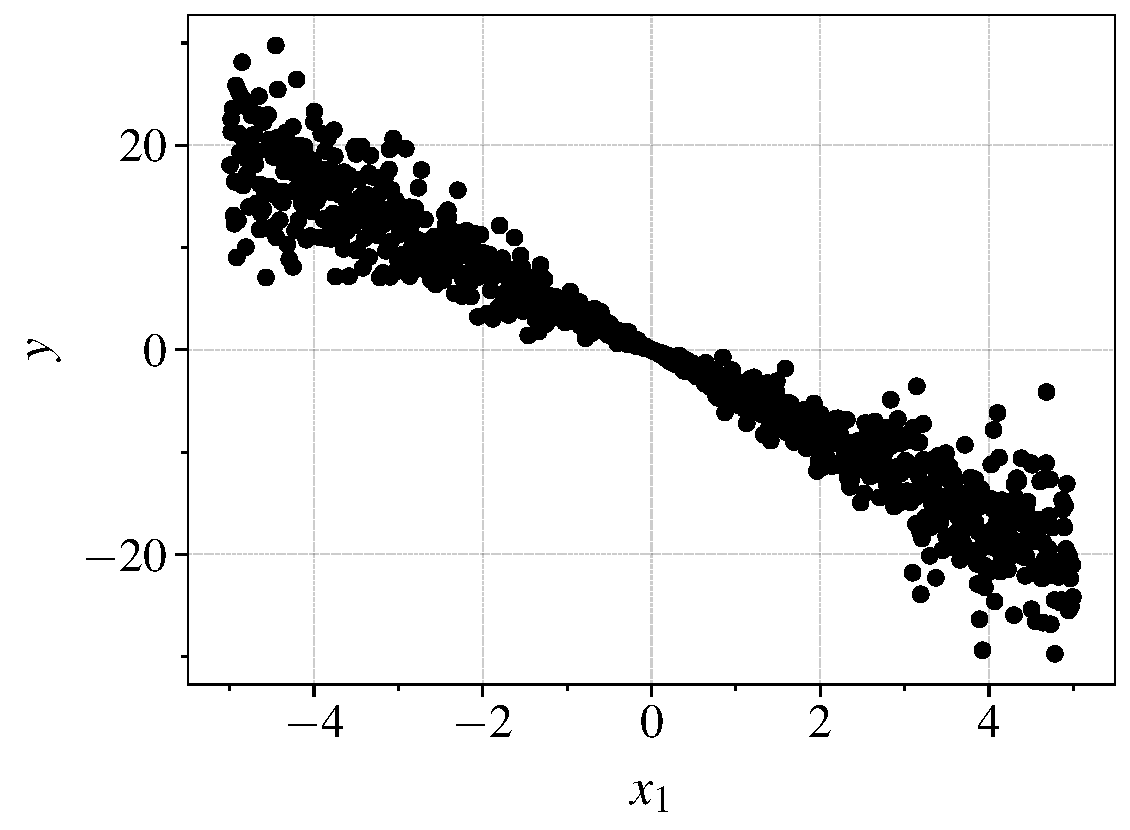
\includegraphics[width=\linewidth]{figures/example_x1_grid.pdf} \\[\abovecaptionskip]
	  \small (a) Scatterplot of $y=f(x_1,x_2)$ and $x_1$.
	\end{tabular}

	\vspace{\floatsep}

	\begin{tabular}{@{}c@{}}
	  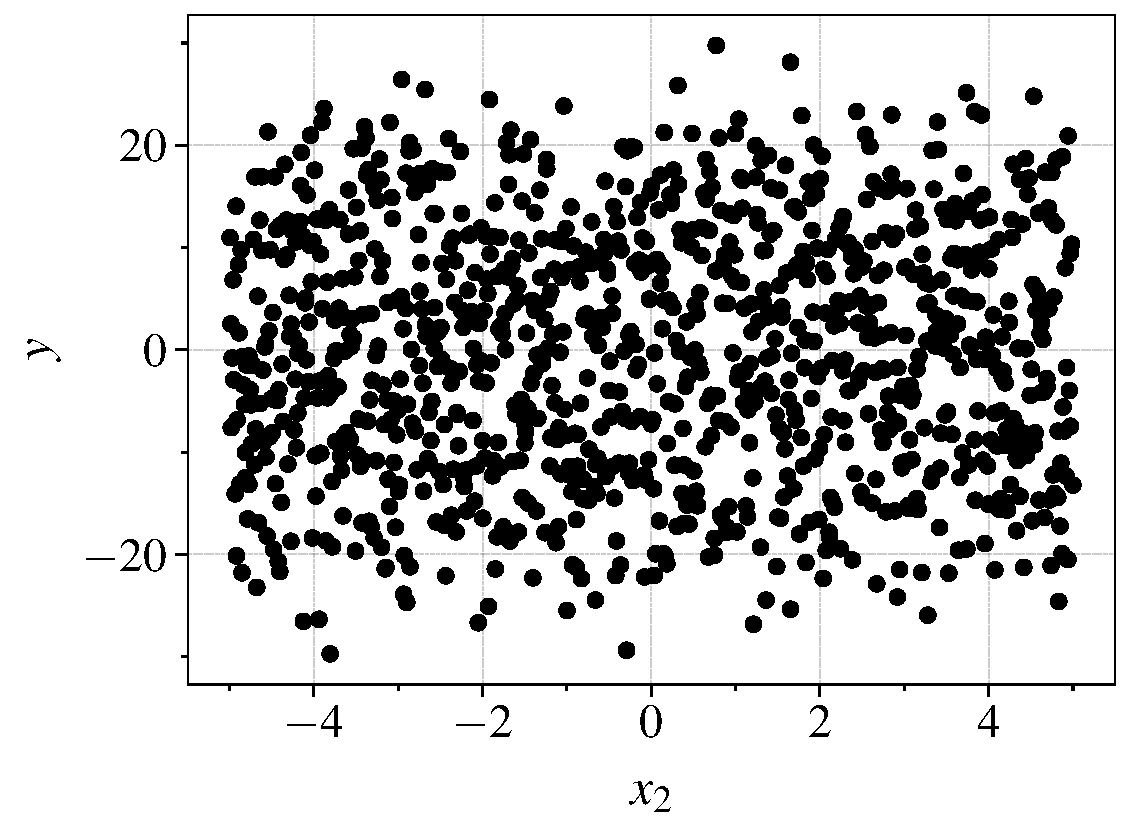
\includegraphics[width=\linewidth]{figures/example_x2_grid.pdf} \\[\abovecaptionskip]
	  \small (b) Scatterplot of $y=f(x_1,x_2)$ and $x_2$.
	\end{tabular}

	\caption{Results of the evaluation of a black-box function $y=f(x_1,x_2)$ with $x_1,x_2 \in [-5,-5]$ using 1000 samples generated with Latin Hypercube sampling.}
	%Function $y$ shows strong dependence with $x_1$, but little or no dependence with $x_2$.}
	\label{fig:myfig}
\end{figure}

The dependence can be captured measuring the area described by the scatterplot, and comparing it to the box defined by $(\underline{y},\overline{y})\times(\underline{x_i},\overline{x_i})$,
where $\underline{y},\overline{y}$ are the measured minimum and maximum of $y$, and $\underline{x_i},\overline{x_i}$ the minimum and maximum of the $i-th$ input parameter.
If the measured area equals to the box area, then it can be said that the output has no dependence on that input.
If the measured area has a value of 0, it means that the output is determined by that input.
Then, any other degree of dependence will fall in-between these two extreme cases.
It is important to note that the measurement of the output area will be an approximation of the actual area, being a consequence of the sampling method or the subintervalization
if interval arithmetic is employed to solve the model functions.
The approximation can be improved increasing the number of samples or subintervals, to the detriment of computational cost.

The sensitivity index is calculated with the following formula

\begin{equation}
	S_i = 1 - \frac{\sum_n^N(\underline{x_i},\overline{x_i})_n\times(\underline{y},\overline{y})_n}{(\underline{y},\overline{y})\times(\underline{x_i},\overline{x_i})}{,}
\end{equation}

where $N$ is the total number of subintervals.
Therefore, $S_i$ is a sensitivity index ranging from 0 (i.e. $y$ is independent of $x_i$) to 1 (i.e. $y$ is determined by $x_i$).

The area can be calculated with two different methods depending on whether interval arithmetic was employed to calculate the functions or it was done though sampling.
In the case of interval arithmetic the calculation is straightforward as the subintervals can be recycled and the rectangles described by these can be easily computed.
On the other hand, if sampling methods were chosen, then the area can be calculated employing an integration method similar to the trapezoidal rule: a step size is defined to
sweep through subintervals of $x_i$ in the data, the minimum $\underline{y}$ and maximum $\overline{y}$ are retrieved for each subinterval, and the rectangle area is computed as usual.
The main drawback of the integration method is that a step size has to be defined manually, and the impact of this parameter on the proposed sensitivity analysis method has not
been studied yet.
However, since the method is similar to the trapezoidal rule, it may be possible to place error bounds on the accuracy of the sensitivity index.

Figure 2 shows how the areas would be calculated from Figure 1  with the sampling approach.
The algorithm requires the output and input data, and the number of subintervals to divide it (20 were used in this example).
Then the minimum and maximum output are found for each subinterval, and the area of the rectangle is calculated.
The total measured area defined by the scatterplot would be the sum of all the rectangles.

\begin{figure}[!b]
	\centering
	\begin{tabular}{@{}c@{}}
	  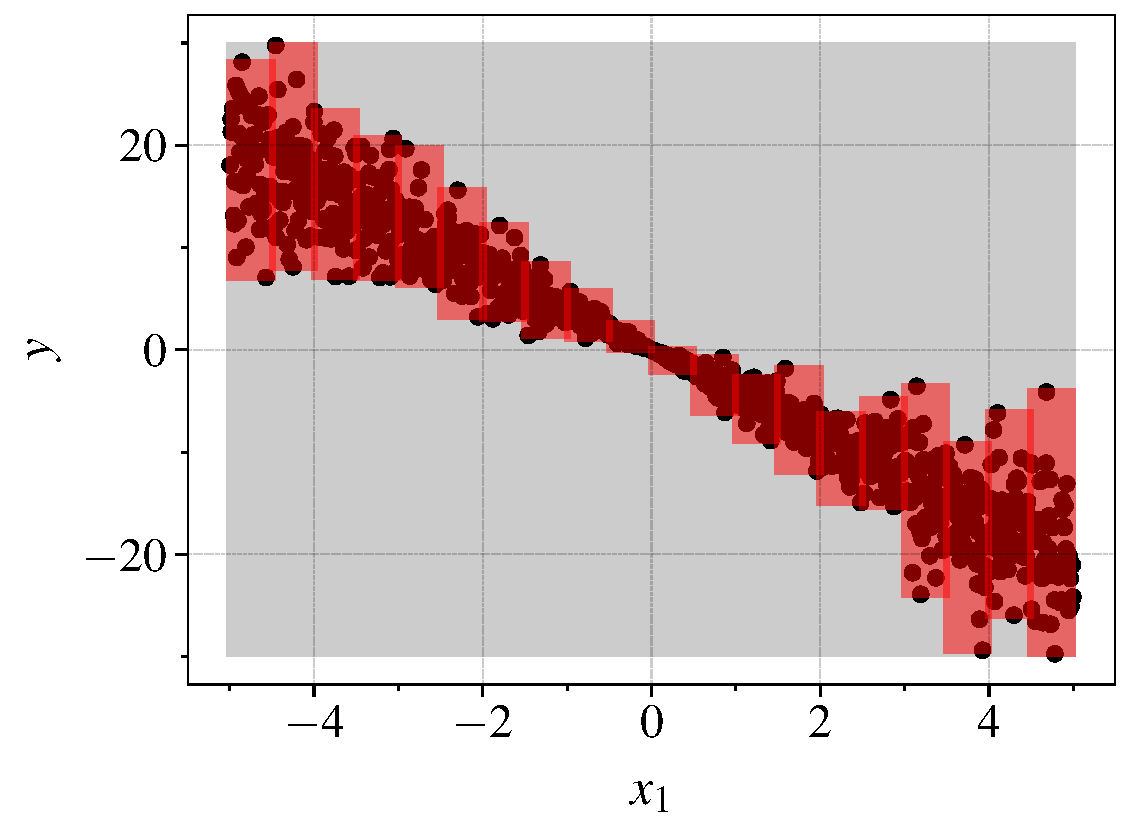
\includegraphics[width=\linewidth]{figures/example_sampling_x1_grid.pdf} \\[\abovecaptionskip]
	  \small (a) Measured scatterplot area (red) and box area (grey)\\
	  \small of $y=f(x_1,x_2)$ and $x_1$.
	\end{tabular}

	\vspace{\floatsep}

	\begin{tabular}{@{}c@{}}
	  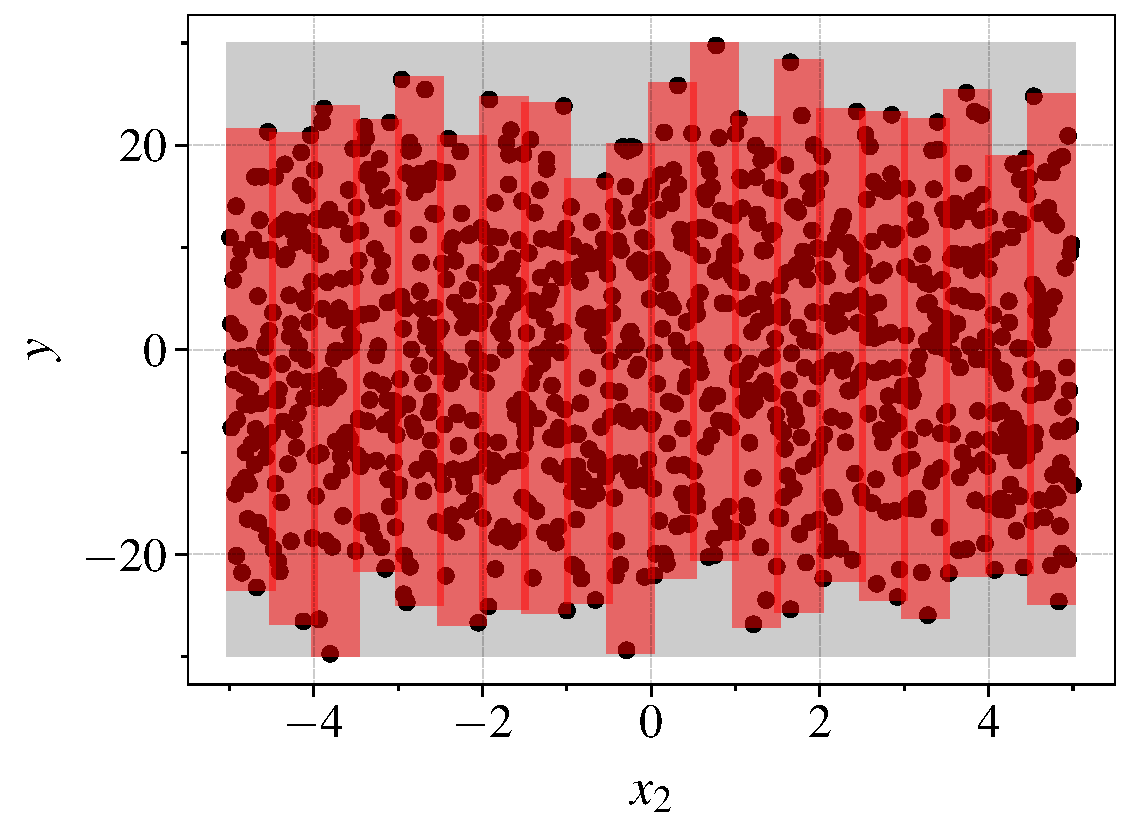
\includegraphics[width=\linewidth]{figures/example_sampling_x2_grid.pdf} \\[\abovecaptionskip]
	  \small (b) Measured scatterplot area (red) and box area (grey)\\
	  \small of $y=f(x_1,x_2)$ and $x_2$.
	\end{tabular}

	\caption{Results of the evaluation of $y=f(x_1,x_2)$ with $x_1,x_2 \in [-5,-5]$ using 1000 samples generated with Latin Hypercube and 20 subintervals.
	The sensitivity index is calculated as in Eq. (1), where the numerator is equal to the area coloured in red and the denominator
	equal to the area coloured in grey.}
	%Function $y$ shows strong dependence with $x_1$, but little or no dependence with $x_2$.}
	\label{fig:myfig}
\end{figure}

Figure 3 shows the 20 subintervals computed with interval arithmetic using the IntervalArithmetic.jl Julia package (\cite{benet2020juliaintervals}).
Note that since the function $y = f(x_1,x_2)$ is a black-box function, the access to its analytical form is restricted, and therefore the
interval arithmetic approach would not be possible.
However, it has been included as an example to show how the interval arithmetic approach would work.

The sensitivity indices for $x_1,x_2$ calculated with the sampling and arithmetic approaches are displayed in Table 1.
Both approaches return the same ordering, indicating that $x_1$ is the dominant parameter.
Note that the interval arithmetic approach captures that $x_2$ has no impact on the uncertainty of $y$ (it also can be seen in Figure 3b, since the
red area equals to the grey area, making $S_2 = 0$), whilst the sampling approach is not that precise.
This is caused by the fact that the sampling approach is an inner approximation method, and the greater the number of samples,
the more accurate the sensitivity index is.

\begin{table}[!h]
	\tbl{Sensitivity indices for $x_1$ and $x_2$ with sampling and arithmetic approaches.}
	{\tabcolsep14pt
	\begin{tabular}{@{}lll@{}}\toprule 
	Index & Sampling & Interval Arithmetic\\
\colrule

	$S_1$ & 0.790 & 0.732\\
	$S_2$ & 0.197 & $\sim0$\\
\botrule
	\end{tabular}}

\end{table}

\begin{figure}[!b]
	\centering
	\begin{tabular}{@{}c@{}}
	  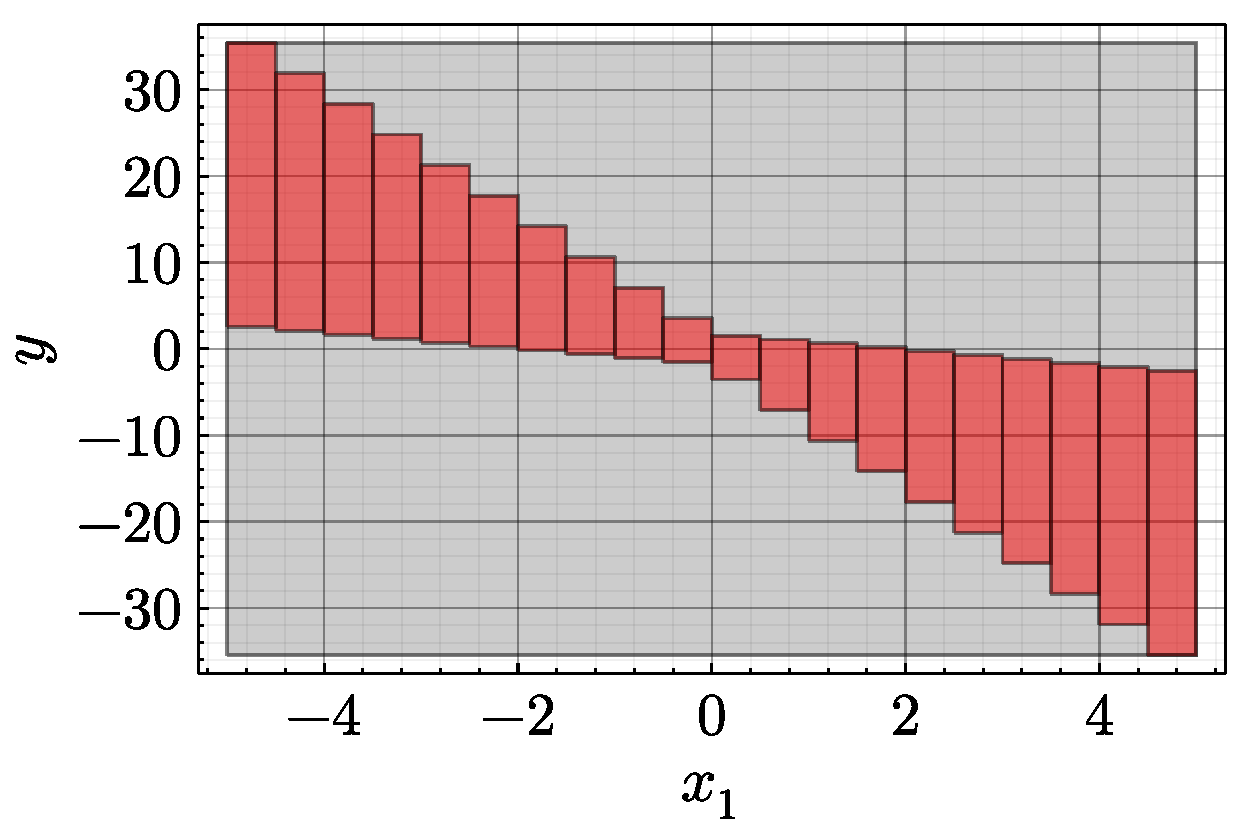
\includegraphics[width=\linewidth]{figures/example_boxes_1.pdf} \\[\abovecaptionskip]
	  \small (a) Visualisation of the 20 subintervals\\
	  \small of $y=f(x_1,x_2)$ and $x_1$.
	\end{tabular}

	\vspace{\floatsep}

	\begin{tabular}{@{}c@{}}
	  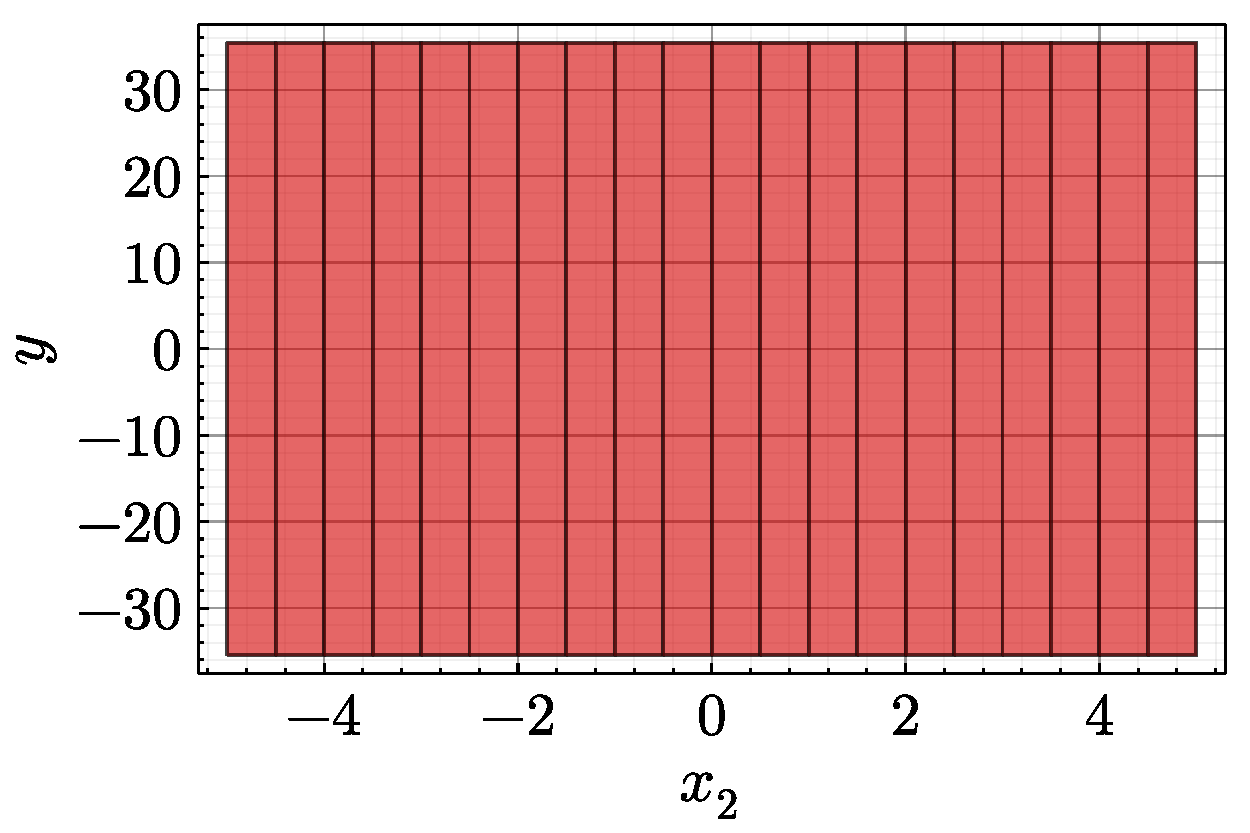
\includegraphics[width=\linewidth]{figures/example_boxes_2.pdf} \\[\abovecaptionskip]
	  \small (b) Visualisation of the 20 subintervals\\
	  \small of $y=f(x_1,x_2)$ and $x_2$.
	\end{tabular}

	\caption{Results of the evaluation of $y=f(x_1,x_2)$ with $x_1,x_2 \in [-5,-5]$ using 20 subintervals and interval arithmetic.
	The sensitivity index is calculated as in Eq. (1), where the numerator is equal to the area coloured in red and the denominator
	equal to the area coloured in grey.}
	%Function $y$ shows strong dependence with $x_1$, but little or no dependence with $x_2$.}
	\label{fig:myfig}
\end{figure}

Lastly, an important by-product of the proposed sensitivity index is that its calculation also entails the so called \textit{pinching} method.
The \textit{pinching} sensitivity analysis calculates the reduction on the output uncertainty when the uncertainty of an input is reduced from the interval to a single value (e.g., see \cite{ferson2006sensitivity, gray2022inference}).
One drawback of this method is that a single value for each input interval has to be chosen (or several values within the interval, with the consequent
increase of computational cost).
However, the interval-based sensitivity index retrieves all the \textit{pinching} information possible for the given number of subintervals; so not only the
output dependence on the input is measured, but also how the input affects the output across its domain.
Figure 4 shows how reducing uncertainty in $x_2$ entails no reduction on the uncertainty of $y$, whilst reducing the uncertainty on $x_1$ has different consequences on the
uncertainty of $y$ depending on the value of $x_1$.
For example, the maximum output uncertainty reduction is obtained pinching at $x_1 = 0$.

\begin{figure}[!b]
	\centering
	\begin{tabular}{@{}c@{}}
	  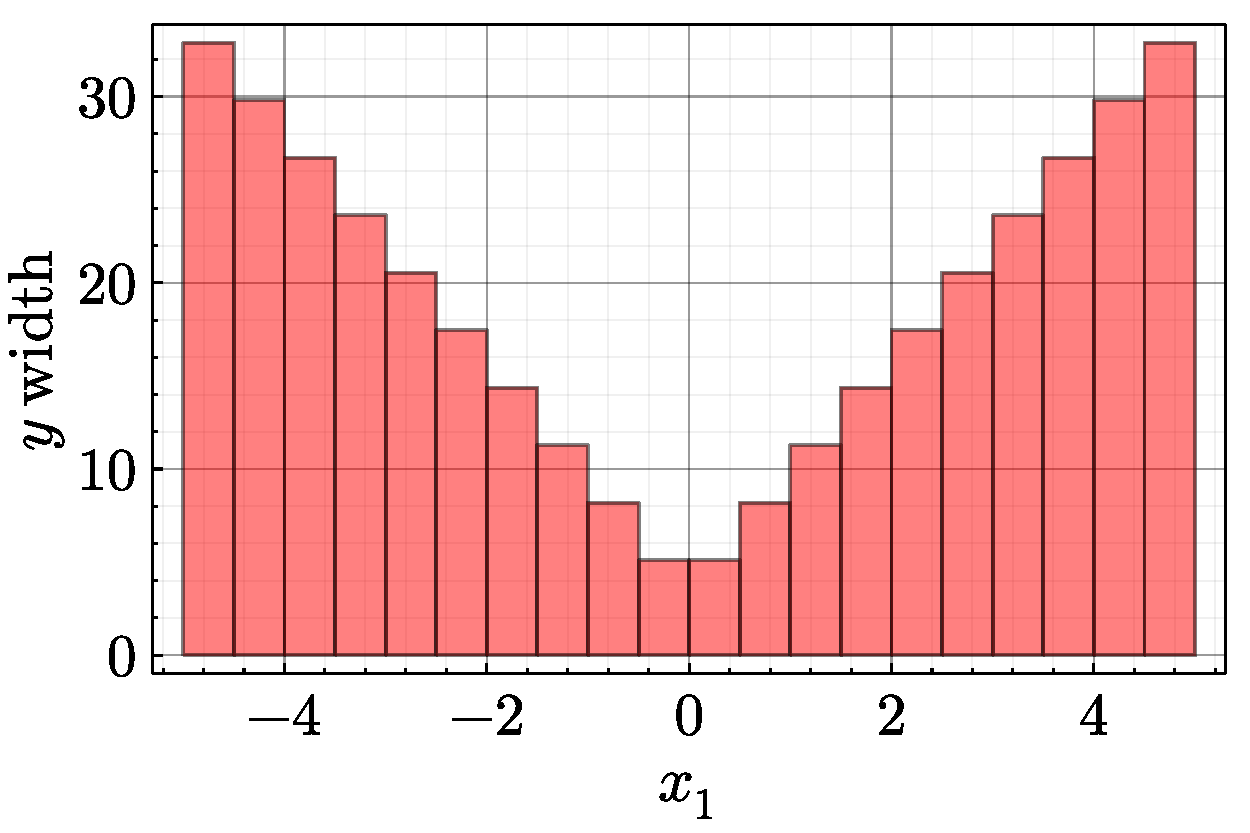
\includegraphics[width=\linewidth]{figures/example_pinching_1.pdf} \\[\abovecaptionskip]
	  \small (a) Output width of $y$ across $x_1$.
	\end{tabular}

	\vspace{\floatsep}

	\begin{tabular}{@{}c@{}}
	  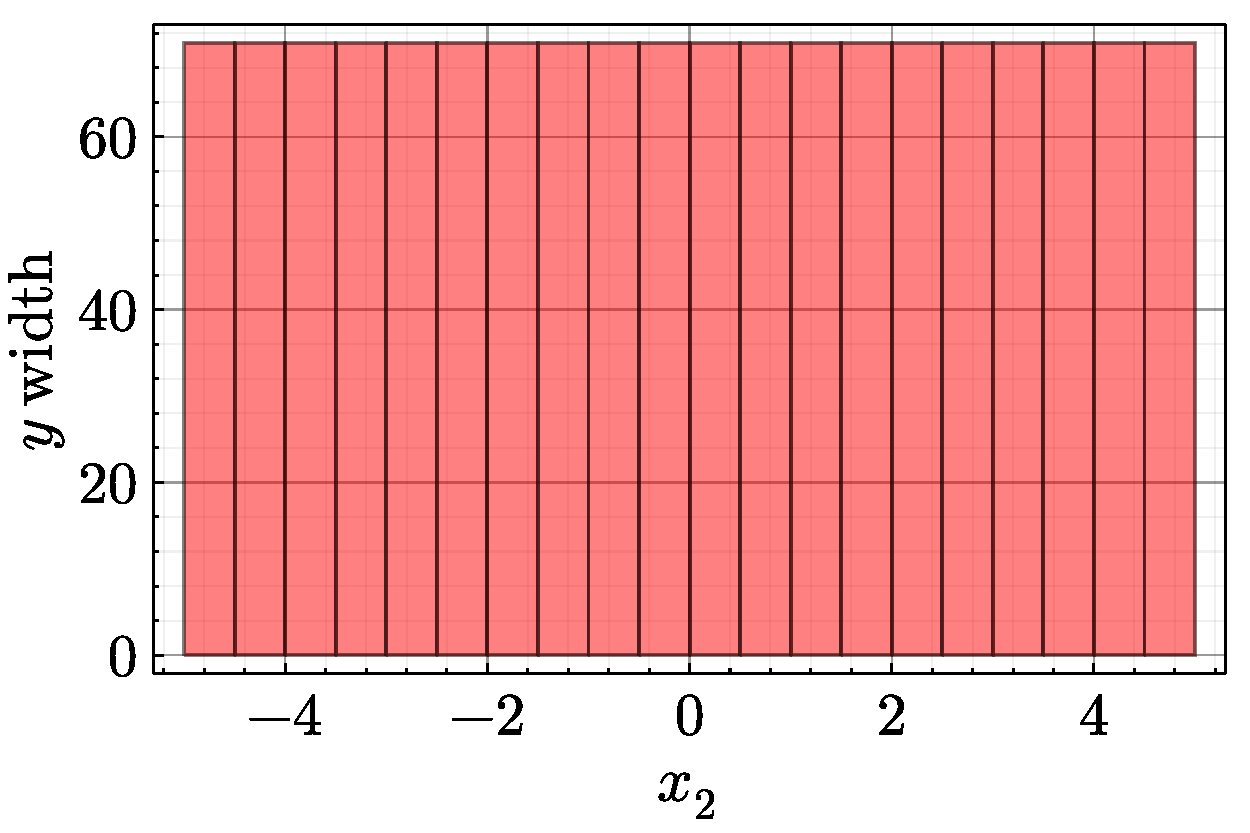
\includegraphics[width=\linewidth]{figures/example_pinching_2.pdf} \\[\abovecaptionskip]
	  \small (a) Output width of $y$ across $x_2$.
	\end{tabular}

	\caption{Output width of $y=f(x_1,x_2)$ across the domain of $x_1$ and $x_2$. This method
	calculates the output uncertainty when reducing the input parameter uncertainty to a subinterval or
	point value.}

\end{figure}

%\begin{enumerate}
%	\item Introduce the area method (overview and illustrating example). [DONE]
%	\item Use example and extreme cases to illustrate (e.g. perfect dependence = index of 1 = no area, independence = index of 0 = all area) [DONE]
%	\item Show equation of the sensitivity index [DONE]
%	\item Explain how it does with arithmetic (subintervalisation) [DONE]
%	\item Explain how it does with sampling (integration similar to trapezoid rule) [DONE]
%	\item Explain pinching. [DONE]
%\end{enumerate}

\section{Application}

To show the performance of the interval-based global sensitivity analysis method proposed, we compare
its results in terms of parameter ranking with the Sobol' indices on the Ishigami function, which is common in the uncertainty quantification
and sensitivity analysis community for its non-linearity, nonmonotonicity, and the interaction effects between $x_1$ and $x_3$ (\cite{ishigami1990importance}).

The Ishigami function can be written as

\begin{equation}
	\centering
	f(x_1,x_2,x_3) = \sin(x_1) + a\sin^2(x_2) + b\sin(x_1)x_3^4{,}
\end{equation}

where the constants are set to $a=5$ and $b=0.1$, and the input variables $x_1,x_2,x_3$ are in $[-\pi,\pi]$.

Since the analytical formula of the function is known, the interval-based sensitivity analysis can be performed with interval
arithmetic.
Figure 5 shows the results of the interval analysis of the Ishigami function with 100 subintervals for $x_1$, $x_2$, and $x_3$, with their corresponding sensitivity
indices indicated in Table 2, calculated following the methodology presented in Section 3.
According to the interval-based method, the Ishigami function has the highest dependence with $x_3$, followed by $x_1$.

\begin{figure}[!b]
	\centering
	\begin{tabular}{@{}c@{}}
	  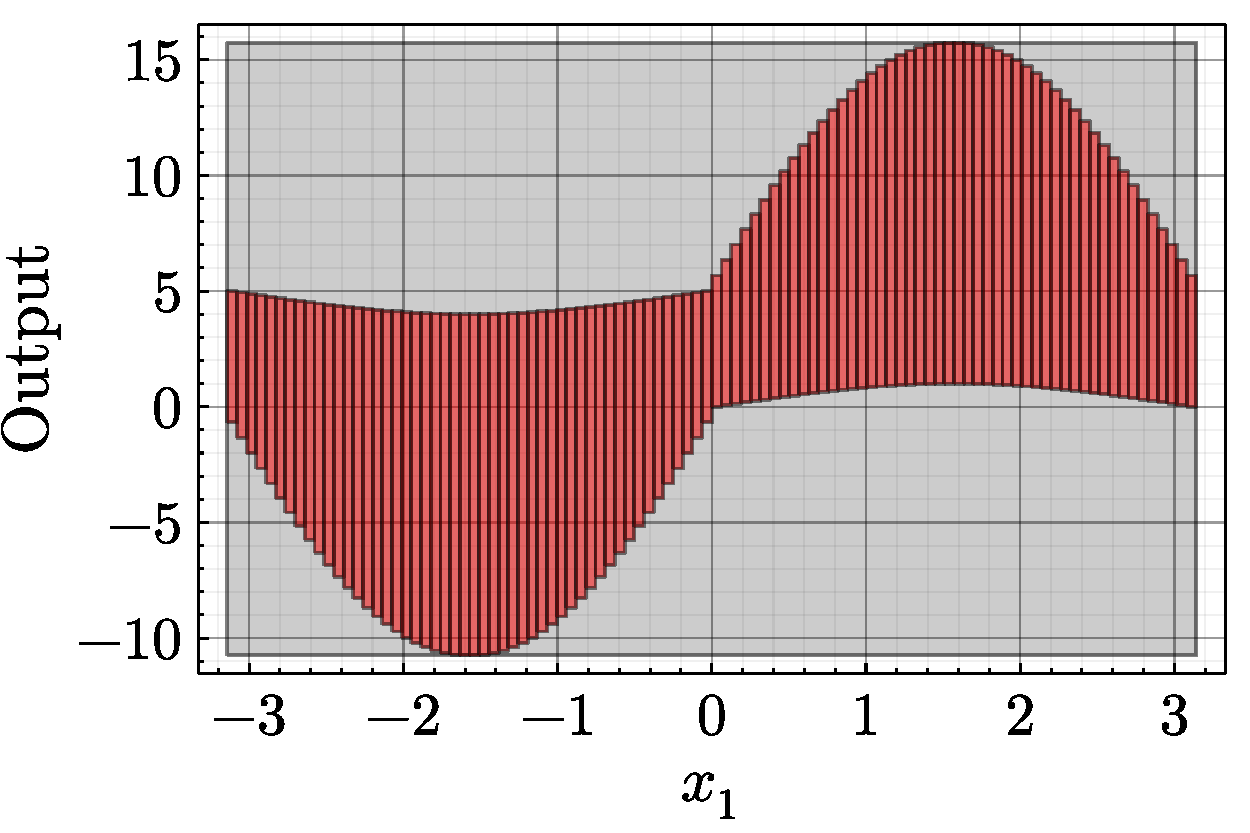
\includegraphics[width=\linewidth]{figures/ishigami_1.pdf} \\[\abovecaptionskip]
	  \small (a) Intervalisation of the Ishigami function\\
	  \small and $x_1$ using 100 subintervals.
	\end{tabular}

	\vspace{\floatsep}

	\begin{tabular}{@{}c@{}}
	  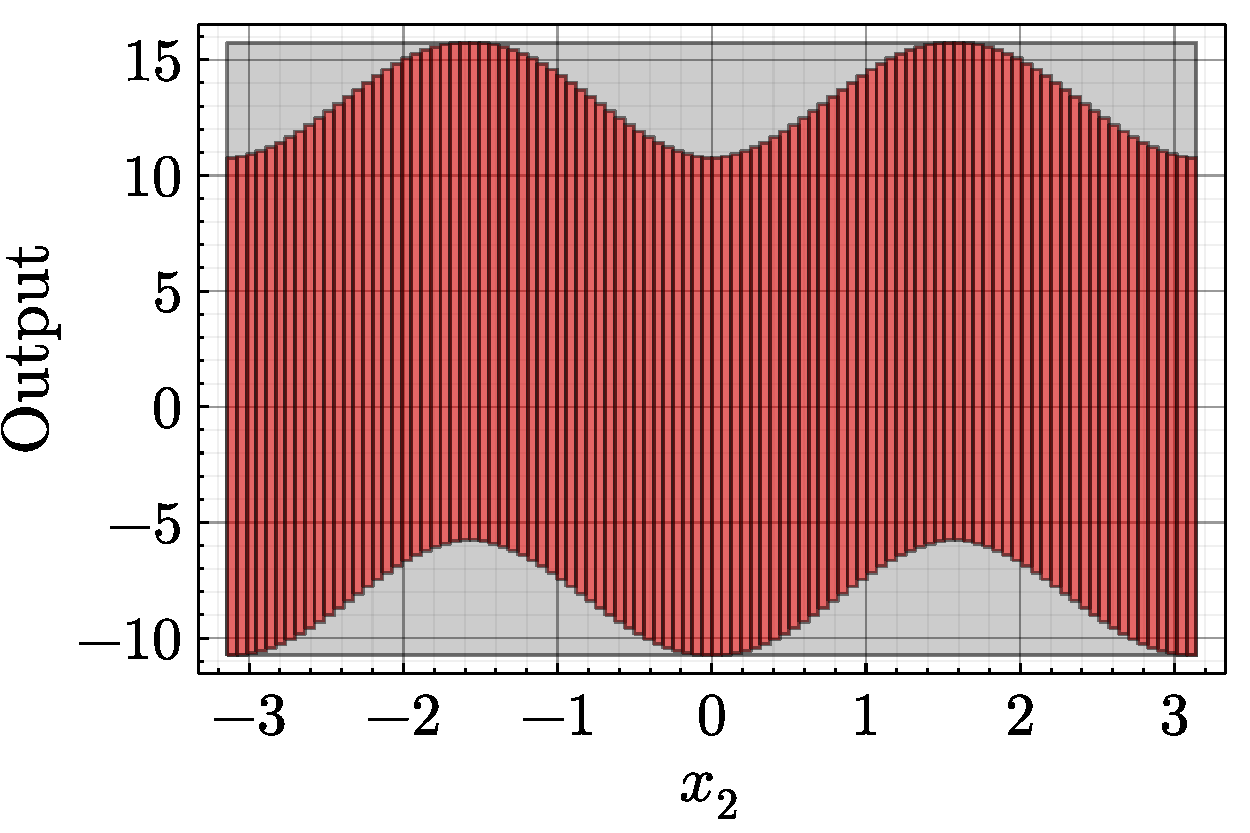
\includegraphics[width=\linewidth]{figures/ishigami_2.pdf} \\[\abovecaptionskip]
	  \small (b) Intervalisation of the Ishigami function\\
	  \small and $x_2$ using 100 subintervals.
	\end{tabular}

	\begin{tabular}{@{}c@{}}
		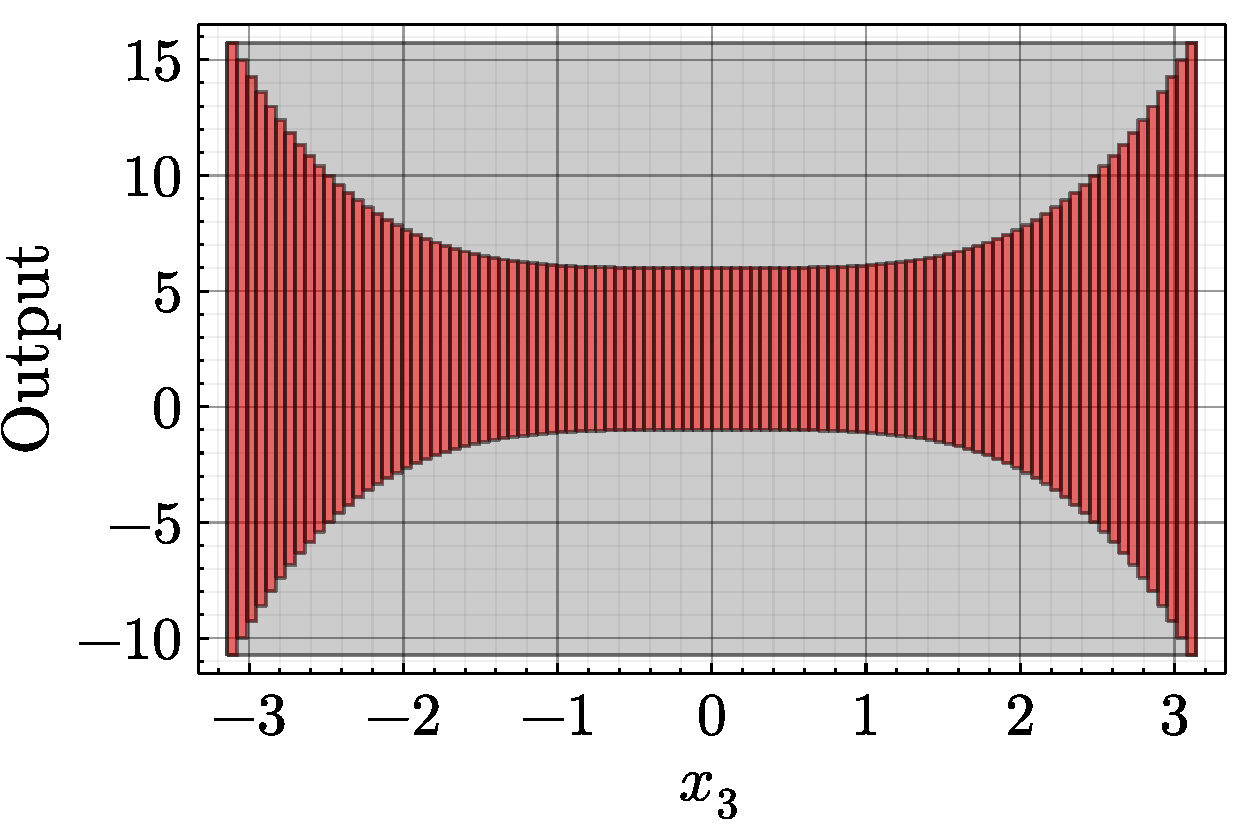
\includegraphics[width=\linewidth]{figures/ishigami_3.pdf} \\[\abovecaptionskip]
		\small (c) Intervalisation of the Ishigami function\\
		\small and $x_3$ using 100 subintervals.
	  \end{tabular}

	\caption{Results of the evaluation of the Ishigami function with $x_1,x_2,x_3 \in [-\pi,\pi]$ with interval arithmetic using 100 subintervals.
	}
\end{figure}

\begin{table}[!h]
	\tbl{Interval-based sensitivity indices of the Ishigami function with $x_1,x_2,x_3 \in [-\pi,\pi]$ using interval arithmetic
	and 100 subintervals.}
	{\tabcolsep14pt
	\begin{tabular}{@{}ll@{}}\toprule
	Index & Interval-Based\\
\colrule

	$S_1$ & 0.568 \\
	$S_2$ & 0.181 \\
	$S_3$ & 0.581 \\
\botrule
\end{tabular}}

\end{table}

In addition to the sensitivity indices, the interval-based approach also provides all the information of the \textit{pinching} analysis.
Figure 6 shows the uncertainty on the Ishigami output when pinching $x_1$, $x_2$, and $x_3$.
The maximum reduction on the Ishigami uncertainty is achieved when $x_1$ is fixed to $-\pi$, $0$, or $pi$.
If pinching any of the three parameters to a point value were not possible, the second best strategy to maximise the output uncertainty
reduction would be to pinch the $x_3$ interval from $[-\pi,\pi]$ to $[-1,1]$, as Figure 6 (c) suggests.
Lastly, pinching $x_2$ entails almost the same uncertainty reduction, and the smallest of the three parameters, across its entire domain.

\begin{figure}[!b]
	\centering
	\begin{tabular}{@{}c@{}}
	  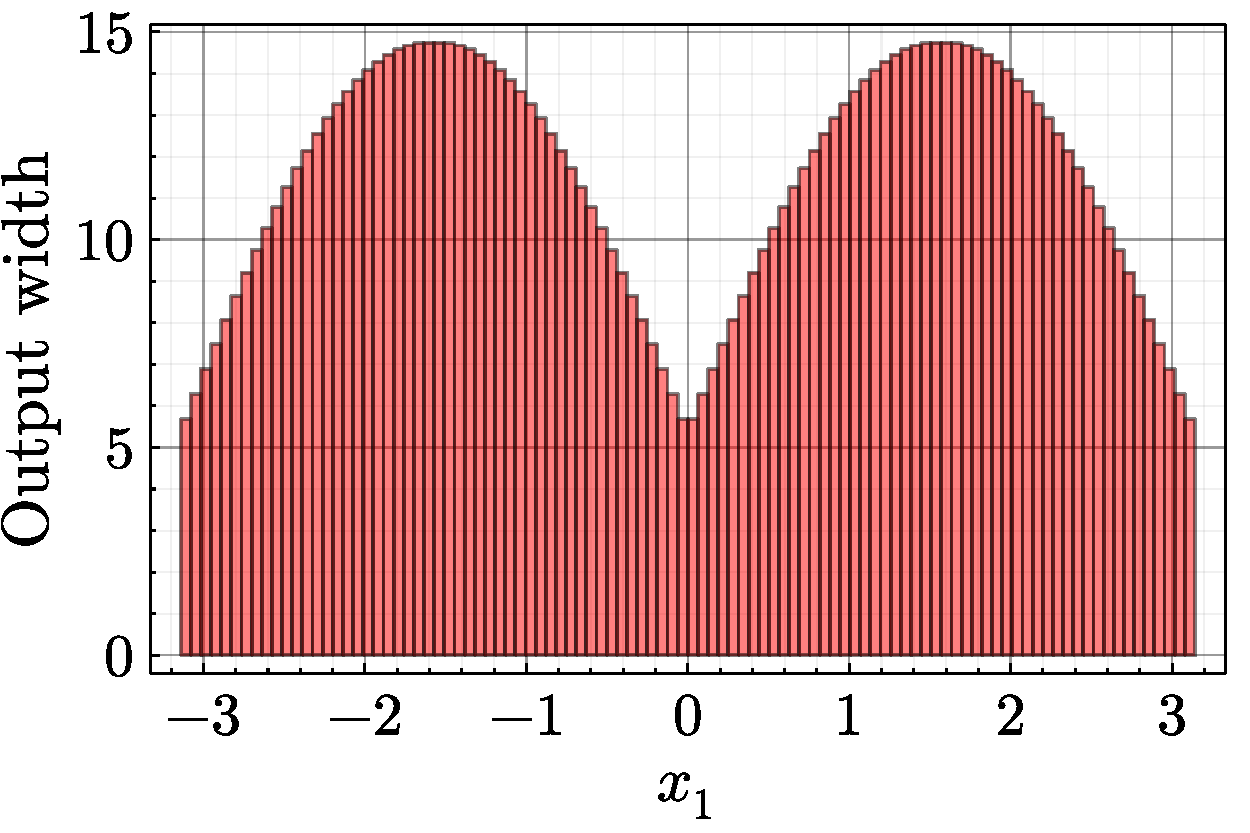
\includegraphics[width=\linewidth]{applications/ishigami_pinching_1.pdf} \\[\abovecaptionskip]
	  \small (a) Output width of the Ishigami function\\
	  \small across $x_1$.
	\end{tabular}

	\vspace{\floatsep}

	\begin{tabular}{@{}c@{}}
	  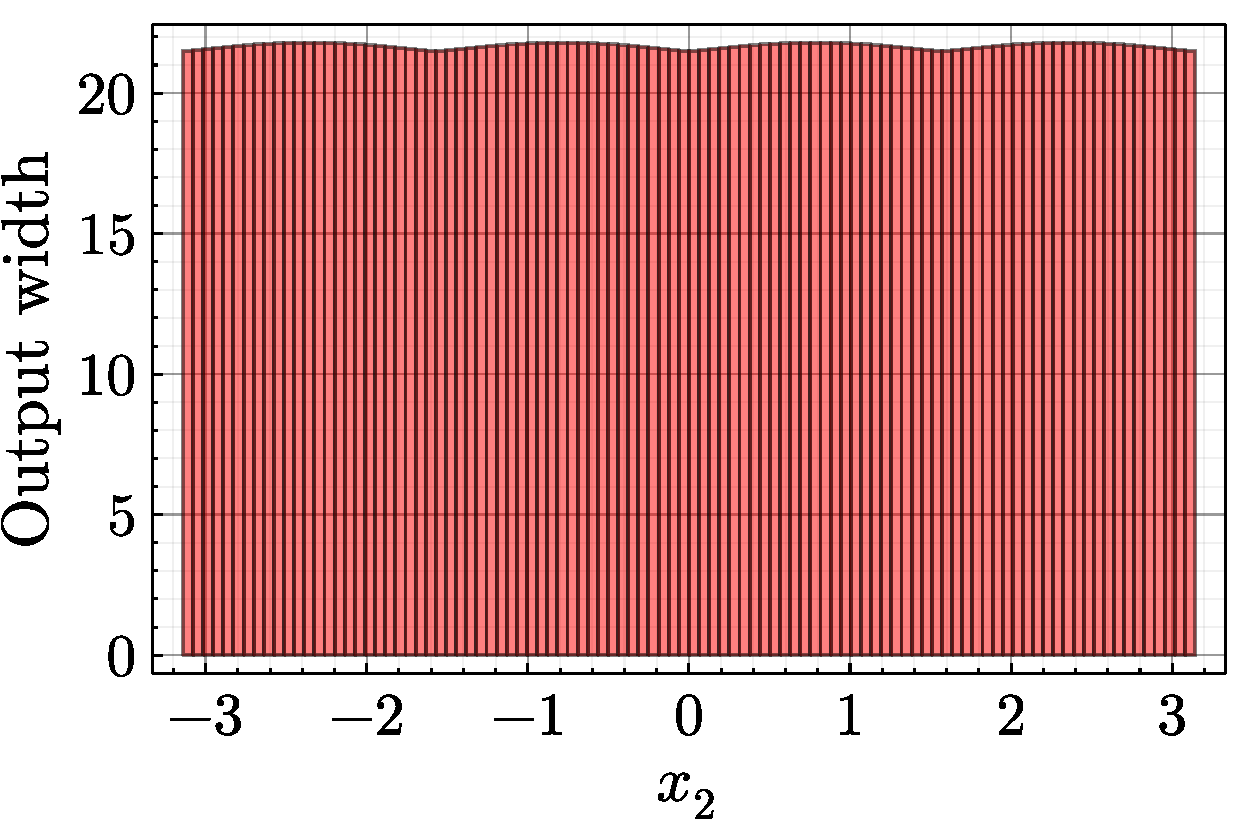
\includegraphics[width=\linewidth]{applications/ishigami_pinching_2.pdf} \\[\abovecaptionskip]
	  \small (b) Output width of the Ishigami function\\
	  \small across $x_2$.
	\end{tabular}

	\begin{tabular}{@{}c@{}}
		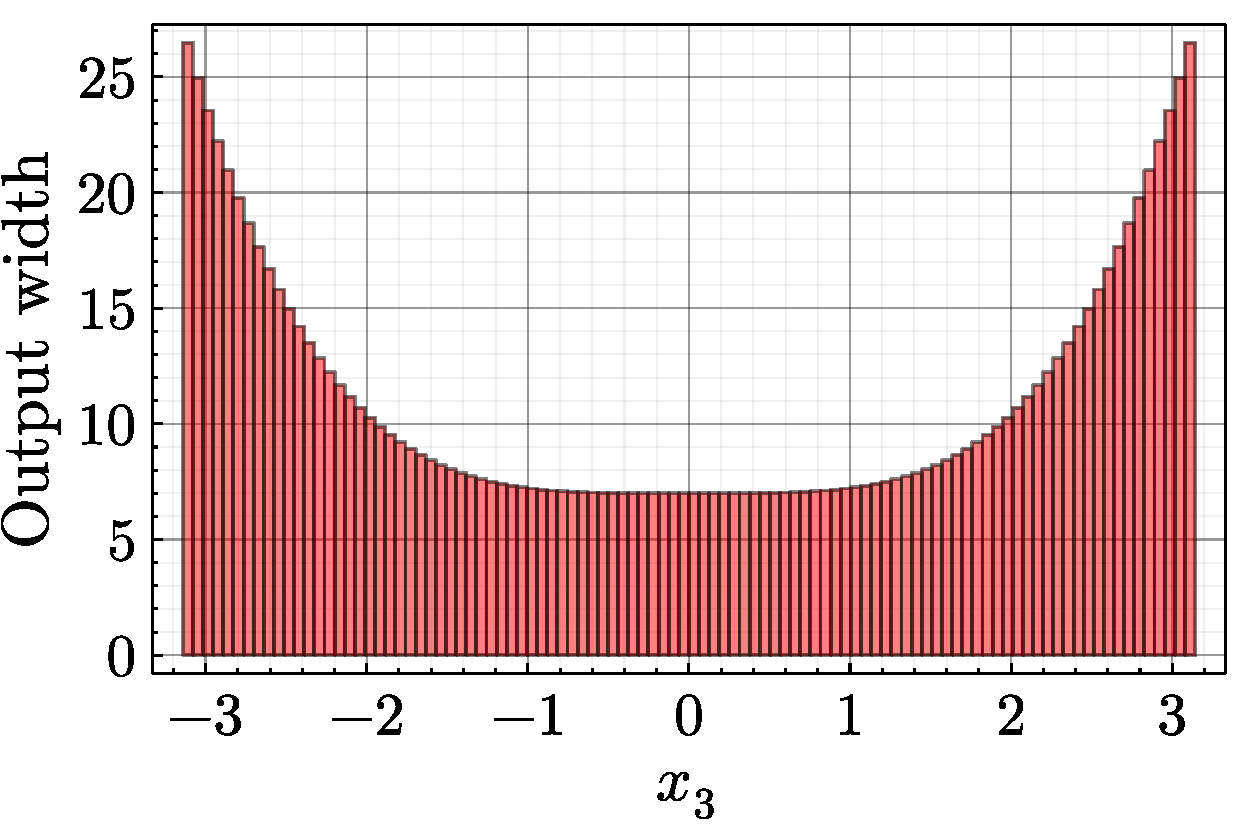
\includegraphics[width=\linewidth]{applications/ishigami_pinching_3.pdf} \\[\abovecaptionskip]
		\small (c) Output width of the Ishigami function\\
		\small across $x_3$.
	  \end{tabular}

	\caption{Output width of the Ishigami function across the domain of $x_1$, $x_2$, and $x_3$.
	}
\end{figure}

When the inputs of the Ishigami function are independent and uniformly distributed in $[-\pi,\pi]$, the analytical description of the variance
terms used to calculate the Sobol' indices are known; therefore the \textit{true} first order and total Sobol' indices can be calculated in this case.
Table 3 contains the analytical Sobol' indices of the Ishigami function.
Analytically, the variance of $x_1$ is the greatest contributor to the variance of the Ishigami function, and $x_3$ has effect on the Ishigami
only when interacting with $x_1$.

\begin{table}[!h]
	\tbl{Analytical first order and total Sobol' indices of the Ishigami function with $x_1,x_2,x_3$ following an uniform distribution in $[-\pi,\pi]$.}
	{\tabcolsep14pt
	\begin{tabular}{@{}lll@{}}\toprule
	Index & First Order & Total\\
\colrule

	$S_1$ & 0.400 & 0.711\\
	$S_2$ & 0.288 & 0.288\\
	$S_3$ & 0.0 & 0.311\\
\botrule
	\end{tabular}}

\end{table}

A second case for the Ishigami function has been included where the input variables follow a triangular distribution in $[-\pi,\pi]$ with mode in $0$
instead of an uniform distribution; this case will support the issue when the distribution functions of the input variables are not totally known, showing
that the Sobol' indices could be sensible to these assumptions.
To calculate the Sobol' indices for the triangular case, 2048 samples were generated using the Saltelli sampling method, which is an extension of the Sobol'
sequence optimised for calculating the indices (\cite{saltelli2002making}).
Table 4 shows the results of the analysis.
The results suggest that, in this case, the variance of $x_2$ is the greatest contributor to the variance of the Ishigami.
Note that the uncertainties on the indices have been omitted since these were negligible, and had no impact on the final parameter ranking.

\begin{table}[!h]
	\tbl{First order and total Sobol' indices of the Ishigami function with $x_1,x_2,x_3$ following a triangular distribution in $[-\pi,\pi]$
	with mode in $0$.}
	{\tabcolsep14pt
	\begin{tabular}{@{}lll@{}}\toprule
	Index & First Order & Total\\
\colrule

	$S_1$ & 0.254 & 0.409\\
	$S_2$ & 0.591 & 0.591\\
	$S_3$ & $\sim0$ & 0.158\\
\botrule
	\end{tabular}}

\end{table}
%\begin{enumerate}
%	\item Explain Ishigami function [DONE]
%	\item Perform IBGSA [DONE]
%	\item Perform Sobol with uniforms[DONE]
%	\item Perform Sobol with triangular [DONE]
%	\item Show pinching. [DONE]
%\end{enumerate}

\section{Discussion}

When the inputs of the Ishigami function are expressed as intervals, without assuming any distribution function,
the interval-based sensitivity analysis claims that $x_3$ is the most important parameter, since the Ishigami function
shows the highest dependence on it, followed by $x_1$.
Sobol' indices where employed in two different cases of the Ishigami function: one where the input were assumed to follow
an uniform distribution in $[-\pi,\pi]$, and in the second case inputs were assumed to follow a triangular distribution
in $[-\pi,\pi]$ with mode at $0$.
In the uniform case, $x_1$ was the first ranked parameter.
On the other hand, in the triangular case, $x_2$ was the first ranked parameter.
These results highlight the fact that variance-based methods for sensitivity analysis can return contradictory results
when the input distribution function cannot be accurately chosen and the variance may not be a reliable statistic.

Furthermore, in the context of digital twins it is important not only to perform parameter priorisation to explain to which
parameter focus the uncertainty reduction, but also to explain how it would be most effective way to reduce output uncertainty.
The results from the interval-based approach suggest that, if reducing input uncertainty to a point value were possible, pinching
$x_1$ to $-\pi$, $0$, or $\pi$ would entail the maximum output uncertainty reduction.
If reducing to a point value were too restrictive (technically, economically...), reducing the uncertainty of $x_3$ from $[-\pi,\pi]$
to $[-1,1]$ would be best option.
Generally, in variance-based methods the output uncertainty reduction is an average reduction of its variance when the variance of certain input
is reduced some \% (e.g., see \cite{allaire2012variance}).
In that regard, intervals may be easier to interpret than variances, and therefore the interval-based approach could offer
an advantage.

Lastly, variance-based methods provide information about interaction effects in the model (as it does with $x_1$ and $x_3$),
and this is a feature that has not been explored with the interval-based approach.
This feature is definitely useful for model diagnostic, and therefore Sobol' indices can be a useful complement to the
interval-based approach.
Generally, it is desirable to include as many sensitivity analysis methods as possible, as these answer to different questions
and can help to better understand the problem under investigation.

%\begin{enumerate}
%	\item Explain results of interval
%	\item discuss what happens with sobol (variance based)
%	\item compare methods (Sobol says which to reduce but does not say how to reduce)
%	\item One could argue both methods are answering two different questions (dependence vs variance), which is true.
%	The objective of this paper is to introduce a sensitivity analysis method with minimum amount of assumptions and reiterate
%	that variance-based methods could return misleading results when the variance is not a reliable statistic.
%	This is the case of scenarios under epistemic uncertainty.
%\end{enumerate}
%Sobol good for interaction effects, IB lacks
%Factor priorisation in terms of variance reduction is a bit confusing.
%When designing stuff it is much straightforward to work with intervals rather than variances.
%"For factor priorisation purposes then, the conclusion that is drawn from the analysis is to focus future research efforts
%on factor x1, since on average once fixed, factor x1 is expected to reduce the variance of Y by the largest amount".
%weird.

\section{Conclusion}

This paper introduces an interval-based method for performing global sensitivity analysis with interval analysis, computed either
via sampling or with interval arithmetic.
This method only requires expressing the input parameter uncertainty in the form of intervals, and therefore is particularly
suited for cases under epistemic uncertainty.
Also, calculating the interval-based sensitivity indices also retrieves all the information of the pinching method,
which measures the output uncertainty reduction when input uncertainty is reduced to a point value or subinterval.
The interval-based approach is applied to the Ishigami function, and its results were compared with the Sobol' indices.
When there is lack of knowledge about the probability distribution function of the inputs (i.e. epistemic uncertainty), variance
based methods such as Sobol' indices may return contradictory results.
This effect was illustrated using uniform and triangular distribution functions for the inputs of the Ishigami.
In this respect, when the inputs are not precisely known the interval-based approach is more reliable since it returns the same
parameter ranking for a given input domain.
This is an initial work towards sensitivity analysis methods for epistemic uncertainty, and further work should be done to better
understand the nature and limitations of the metric presented in this paper.

%\begin{enumerate}
%	\item Brief recap (we show a SA method blabla..) [DONE]
%	\item Method for epistemic uncertainty (no assumptions) [DONE]
%	\item This method can be used with interval arithmetic or sampling (blackbox) [DONE]
%	\item Compare its performance with Sobol on the Ishigami (sobol good for interaction) [DONE]
%	\item Further work [DONE]
%\end{enumerate}

\begin{acknowledgement}
TBD
\bibliographystyle{chicago}
\bibliography{References}
\end{acknowledgement}


\end{document}




